\PassOptionsToPackage{unicode=true}{hyperref}
\documentclass[
    14pt,
    xcolor=dvipsnames,
    aspectratio=169
]{beamer}

\usepackage{fontspec}
\setsansfont{Lato}
\usefonttheme{professionalfonts}

%% Преамбула.
\usepackage{ragged2e}
\usepackage{color}
\usepackage{epstopdf}

% Ссылки.
%\usepackage[unicode=true]{hyperref}

% Улучшенные сноски.
\usepackage{footmisc}

% Продвинутые формулы.
\usepackage{amsmath}
\usepackage{amsfonts}
\usepackage{mathtools}

% Продвинутые математические символы.
\usepackage{amssymb}

% Кастомизируемые теоремы.
\usepackage{amsthm}
%\usepackage{thmtools}

% Русский язык.
\usepackage{cmap}
\usepackage[english, russian]{babel}

% Нижнее подчёркивание с переносами.
\usepackage[normalem]{ulem}

% Графики gnuplot.
\usepackage[shell, subfolder, cleanup]{gnuplottex}

% Работа с плавающими объектами.
\usepackage[section]{placeins}

% Обтекаемые изображения
\usepackage{wrapfig}

% Ячейки на несколько строк.
\usepackage{multirow}
\usepackage{makecell}

% Таблица с регулируемой шириной столбцов и работающими сносками.
\usepackage{tabularx}

% Графика TikZ
\usepackage{tikz}
\usepackage{gnuplot-lua-tikz}


\usepackage[doi=false, isbn=false, url=false, eprint=false, backend=biber, style=gost-numeric]{biblatex}
\usepackage{csquotes}

\addbibresource{references.bib}

%% Определения команд.
%% Математические символы и прочие дефайны.

\def\defarr{\overset{\triangle}{\Longleftrightarrow}} % <<По определению>>
\def\defeq{\triangleq}                                % <<По определению равно>>
\def\symdiff{\,\triangle\,}                           % <<Симметрическая разность>>
\def\connected{\leftrightsquigarrow}                  % Связность в графах.
\def\optimal{\star}                                   % Оптимальное значение.

% Большая черта в множествах.
\def\Mid{\;\middle|\;}

% Стрелки для сходимостей.
\newcommand{\limarrow}[2][\longrightarrow]{\underset{#2}{#1}}
\newcommand{\limto}[2]{\limarrow{#1 \to #2}}


% Математическое операторы.
\DeclareMathOperator{\diam}{\mathrm{diam}}
\DeclareMathOperator{\rad}{\mathrm{rad}}
\DeclareMathOperator*{\argmin}{\arg\min}
\DeclareMathOperator*{\argmax}{\arg\max}
\DeclareMathOperator*{\dom}{\mathrm{dom}}
\DeclareMathOperator*{\range}{\mathrm{range}}
\DeclareMathOperator*{\closure}{\mathrm{cl}}
\DeclareMathOperator*{\trace}{\mathrm{tr}}
\DeclareMathOperator*{\lowlim}{\underline{lim}}
\DeclareMathOperator*{\uplim}{\overline{lim}}

\newcommand{\mean}[1]{\left\langle #1 \right\rangle} % Усреднение.

% Математические множества.
\def\naturals{\mathbb{N}}  % Натуральные числа.
\def\integers{\mathbb{Z}}  % Целые числа.
\def\rationals{\mathbb{Q}} % Рациональные числа.
\def\reals{\mathbb{R}}     % Действительные числа.
\def\complexes{\mathbb{C}} % Комплексные числа.

%% Функции
\def\blankarg{\,\cdot\,}

%% Линейная алгебра.
\def\diag{\operatorname{diag}} % Диагональная матрица.

%% Функциональный анализ.
\def\banachspace{\mathcal{B}}                                  % Банахово пространство.
\def\hilbertspace{\mathcal{H}}                                 % Гильбертово пространство.
\def\linopset{\mathcal{L}}                                     % Множество линейных ограниченных операторов.
\newcommand{\dotprod}[2]{\left\langle #1, #2 \right\rangle}    % Скалярное произведение.
\def\identity{\mathrm{I}}                                      % Единичный оператор.

%% Комплексные числа.
\def\Re{\operatorname{Re}} % Действительная часть.
\def\Im{\operatorname{Im}} % Мнимая часть.

%% Асимптотические классы.
\def\Oclass{\mathcal{O}} % О-большое.

%% Выделение определения.
\DeclareTextFontCommand{\defemph}{\bfseries\em}


%% Теория вероятностей.
%% Теория вероятностей.
\def\proba{\mathbb{P}}
\def\setfamily{\mathcal{F}}
\def\borel{\mathcal{B}}
\def\trajectories{\mathcal{X}}
\def\indicator{\mathbb{I}}
\def\lebesgue{\mathbb{L}}
\def\iid{\textnormal{н.о.р.с.в.}}

% Моменты.
\DeclareMathOperator{\expect}{\mathbb{E}}
\DeclareMathOperator{\dispersion}{\mathbb{D}}
\newcommand{\covariance}[2]{\textnormal{cov}\left(#1, #2\right)}
\newcommand{\rvcenter}[1]{\mathring{#1}}

% Распределения.
\def\bernoulli{\textnormal{Be}}
\def\binomial{\textnormal{Bi}}
\def\poisson{\textnormal{Po}}
\def\uniform{\textnormal{U}}
\def\expdistr{\textnormal{Exp}}
\def\normal{\mathcal{N}}

% Сходимости.
\DeclareMathOperator*{\limmeansq}{\textnormal{l.i.m.}}
\newcommand{\converges}[1]{\overset{#1}{\longrightarrow}}
\def\convmeansq{\converges{\textnormal{с.к.}}}
\def\convalmost{\converges{\textnormal{п.н.}}}
\def\convproba{\converges{\proba}}
\def\convdistr{\converges{d}}
\def\convnorm{\converges{\| \cdot \|}}

\def\almosteq{\overset{\textnormal{п.н.}}{=}}
\def\distreq{\overset{d}{=}}


%% Численные методы.
%% Численные методы.
\def\res{\mathcal{R}}              % Невязка
\def\jac{\mathcal{J}}              % Матрица Якоби
\newcommand{\bvec}[1]{\mathbf{#1}} % ``Жирный'' вектор.
\def\stabreg{\mathbf{R}}           % Область устойчивости.
\def\niter{N_{\text{итер}}}        % Число итераций.
\def\abseps{\varepsilon_{\text{абс}}} % Абсолютная погрешность.
\def\releps{\varepsilon_{\text{отн}}} % Относительная погрешность.

\newcommand{\lognorm}[1]{\mu \left[ #1 \right]} % Логарифмическая норма.

\def\taulin{\tau_{\textnormal{лин}}}      % Характерное время линейной реакции системы на возмущения.
\def\taunonlin{\tau_{\textnormal{нелин}}} % Характерное время, за которое меняется матрица Якоби правой части системы.
\def\taudiss{\tau_{\textnormal{дисс}}}      % Характерное время диссипации.

\def\nmfamily{\mathcal{F}_{\textnormal{NM}}} % Семейство численных схем.
\def\rhsfamily{\mathcal{F}_{\textnormal{RHS}}} % Семейство правых частей ДУ.
\def\initialcond{\banachspace_0} % Множество допустимых начальных значений.


%% Определение сред.
%%% Счётчик для теорем.
\newcounter{TheoremCounter}
\counterwithin{TheoremCounter}{chapter}

%% Теоремы.
\newtheorem{theorem}[TheoremCounter]{Теорема}
\newtheorem{lemma}[TheoremCounter]{Лемма}
\newtheorem{corollary}[TheoremCounter]{Следствие}
\newtheorem{definition}[TheoremCounter]{Определение}
\newtheorem{remark}[TheoremCounter]{Замечание}
\newtheorem{statement}[TheoremCounter]{Утверждение}
\newtheorem{problem}[TheoremCounter]{Задача}
\newtheorem{example}[TheoremCounter]{Пример}


%% Список литературы.
\addbibresource{references.bib}

\setlength{\parskip}{0.25\baselineskip}
\setbeamerfont{footnote}{size=\tiny}
\justifying

\mode<presentation>
{
    %\usetheme{Madrid}
    %\usetheme{Warsaw}
    %\usecolortheme{lily}
    %\usecolortheme{structure}

    %\useoutertheme[subsection=false]{smoothbars}
    %\useinnertheme{rounded}
    \setbeamertemplate{navigation symbols}{}
    \setbeamertemplate{headline}{}
    \setbeamertemplate{footline}
    {
        \leavevmode%
        \hbox{%
        \begin{beamercolorbox}[wd=.4\paperwidth,ht=2.25ex,dp=1ex,center]{author in head/foot}%
            \usebeamerfont{author in head/foot}\insertshortauthor
        \end{beamercolorbox}%
        \begin{beamercolorbox}[wd=.5\paperwidth,ht=2.25ex,dp=1ex,center]{title in head/foot}%
            \usebeamerfont{title in head/foot}\insertshorttitle
        \end{beamercolorbox}}%
        \begin{beamercolorbox}[wd=.1\paperwidth,ht=2.25ex,dp=1ex,center]{author in head/foot}%
            \insertframenumber{} / \inserttotalframenumber
        \end{beamercolorbox}
    }%
    \vskip0pt%
}

\setbeamertemplate{itemize items}[triangle]
\setbeamertemplate{enumerate items}[square]
\setbeamertemplate{caption}[numbered]

\setbeamerfont{title}{size=\large,parent=structure}

\definecolor{Sirius}{rgb}{0.004, 0.616, 0.631}
\usecolortheme[named=Sirius]{structure}

\title[Выпускная квалификационная работа магистра]{Исследование процессов тромбообразования при помощи математических моделей}


\author[Иван Бутаков, М01ММ-22]{
    Бутаков Иван Дмитриевич\\
    {\scriptsize \tt \href{mailto:butakov.id@phystech.edu}{butakov.id@phystech.edu}}\\
    \vspace{\baselineskip}
    {\small Научный руководитель: Терехов Кирилл Михайлович, к.ф.-м.н.}%
}

\institute[НТУ <<Сириус>>]{
    \vfill
    %\insertlogo\\
    НТУ <<Сириус>>\\ Математическое моделирование в биомедицине и геофизике%
}

\date{{\scriptsize 06.07.2024}}

%\logo{
\includegraphics[width=1.5cm]{images/Sirius-logo.png}}


\AtBeginSection[]
{
    \begin{frame}[noframenumbering]
        \frametitle{Содержание}
        \tableofcontents[currentsection,hideothersubsections]
    \end{frame}
}

%\usepackage{caption}
%\captionsetup{font=scriptsize,labelfont=scriptsize}
\setbeamerfont{caption}{size=\small}

\begin{document}

\begin{frame}
    \titlepage
\end{frame}

%\begin{frame}
%    \frametitle{Содержание}
%    \tableofcontents[hideallsubsections]
%\end{frame}

\section{Актуальность и постановка задачи}

\begin{frame}{Акутальность}
    \begin{columns}[T]
        %\Large
        \begin{column}{0.5\textwidth}
            \only<1>{
                \begin{itemize}
                    \item Значительная доля всех смертей вызвана тромбами (инсульт — 2ое место в мире).%
                        \footnote{\textcite{geoffrey2008stroke, who2020global_health_estimates}}
                    \item Вредно давать большие дозы антикоагулянтов, но рисковать нельзя.
                \end{itemize}
            }
            \only<2>{
                Требуется уметь
                \begin{itemize}
                    \item выявлять людей в группе риска;
                    \item рассчитывать минимально эффективную дозу антикоагулянтов.
                \end{itemize}
            }
        \end{column}
        \begin{column}{0.5\textwidth}
            \centering
            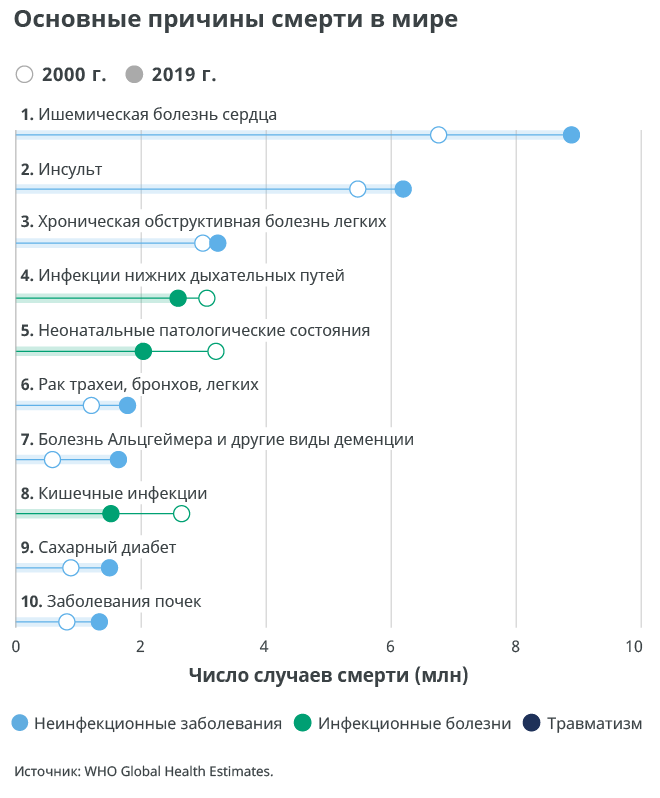
\includegraphics[width=0.8\textwidth]{./images/slides/death_chart.png}
        \end{column}
    \end{columns}
\end{frame}

\begin{frame}{Цель}
    Разработать \textbf{математическую модель} (СОДУ), описывающую два основных механизма образования тромба:
    \begin{itemize}
        \item повреждения тканей (\textbf{<<красный тромб>>});
        \item особенности потока крови (\textbf{<<белый тромб>>}).
    \end{itemize}

    Разработать \textbf{метод численного интегрирования} полученной модели.
\end{frame}

\begin{frame}{Постановка задачи}
    Особенности модели:
    \begin{itemize}
        \item персонификация;
        \item инициация тромбообразования вследствие особых характеристик потока;
        \item учёт антикоагулянтов.
    \end{itemize}

    Особенности численного метода:
    \begin{itemize}
        \item устойчивость;
        \item надёжность в случае нелинейно жёстких систем.
    \end{itemize}
\end{frame}

\section{Модель фибринового тромба}

\begin{frame}{\secname}
    Основа~--- уравнение \textbf{переноса"=диффузии"=реакции}:
    \[
        \frac{\partial \bvec{x}_i}{\partial t} = \mathrm{div} (D \nabla \bvec{x}_i) - \mathrm{div} (\vec{v} \bvec{x}_i) + \bvec{R}_i
    \]
\end{frame}

\begin{frame}{\secname}
    \begin{columns}[T]
        \begin{column}{0.4\textwidth}
           \begin{itemize}
               \item 9 компонент против 40+ в реальной жизни
               \item моделирует только <<красный тромб>>
           \end{itemize}
        \end{column}
        \begin{column}{0.6\textwidth}
            \centering
            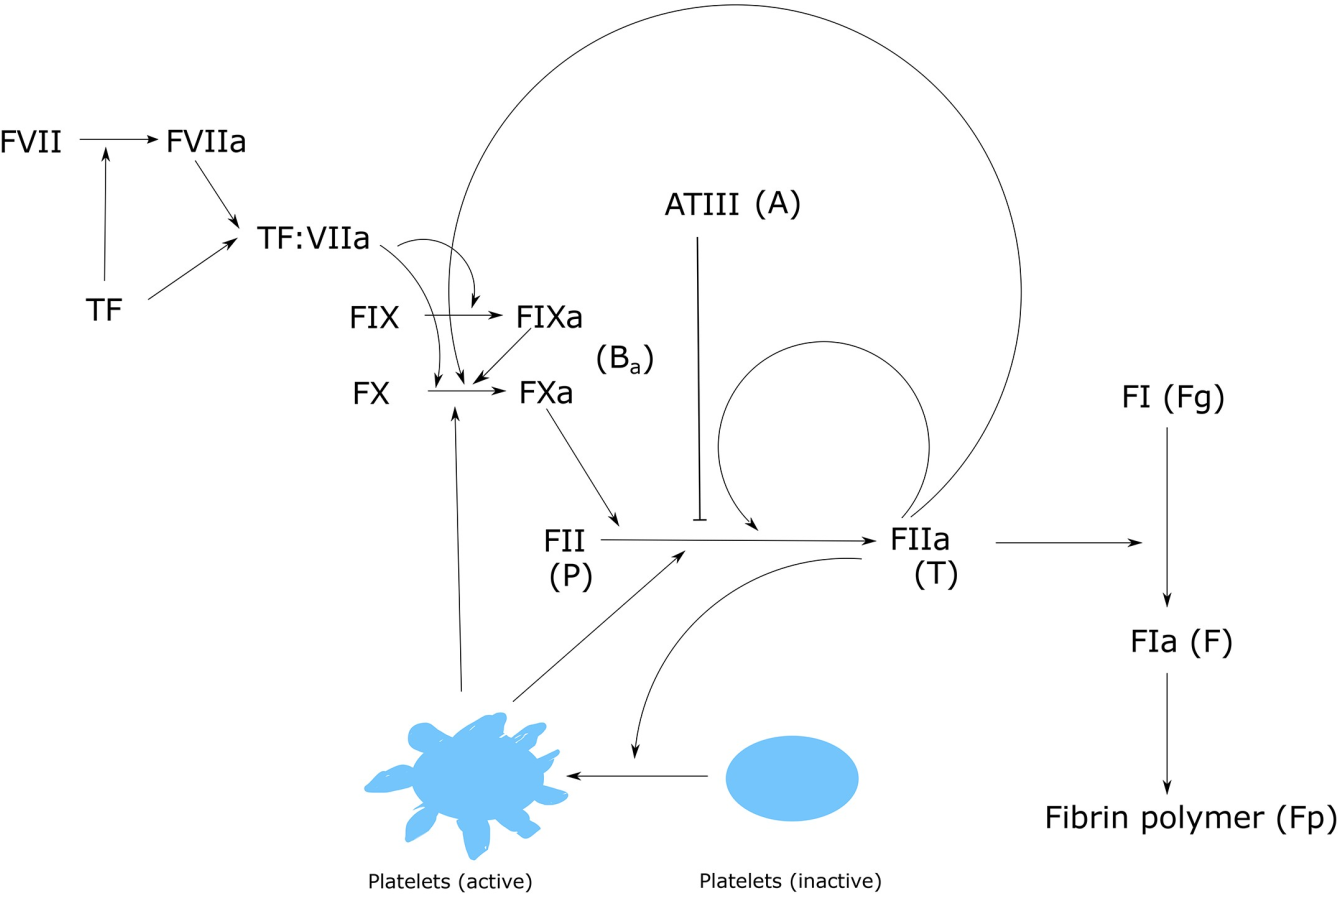
\includegraphics[width=1.0\textwidth]{./images/slides/model.png}
        \end{column}
    \end{columns}
\end{frame}

\begin{frame}{\secname}
    Ограничения:
    \begin{itemize}
        \item не воспроизводит тромбоцитарный тромб;
        \item не учитывает механизмы формирования тромбоцитарного тромба;
        \item тромб полагается стационарным.
    \end{itemize}
\end{frame}


\section{Модель тромбоцитарного тромба}

\subsection{Обзор актуальных проблем и задач}

\begin{frame}{\subsecname}
    \begin{itemize}
        \item Решающий фактор инициации тромбообразования~---
            сдвиговые напряжения и другие особые характеристики потока~\cite{lauren2015high_shear_rate_thrombosis, avtaeva2022vWF}.
        \item Решающий фактор роста тромба~--- слипание тромбоцитов~\cite{rasche2001haemostasis_overview, lauren2015high_shear_rate_thrombosis, mereuta2021white_clots}.
        \item На этапе формирования тромб подвижный~\cite{savage1996platelet_adhesion,jamiolkowski2016visualization},
            вязкий~\cite{jamiolkowski2016visualization},
            пластичный~\cite{jamiolkowski2016visualization}.
        \item Тромб пористый~\cite{wufsus2013clot_permeability}.
    \end{itemize}
\end{frame}

\begin{frame}{\subsecname}
    Механизмы разворачивания фактора фон Виллебранда:
    \begin{itemize}
        \item Действие сдвигового напряжения~\cite{lippok2016vWF_unfolding, schneider2007vWF_unfolding, zlobina2016vWF_unfolding, pushin2020vWF_unfolding}.
        \item<1-> <<Сильное разворачивание>> в определённых потоках при большом числе Вайсенберга~\cite{zhussupbekov2021vWF_unfolding}.
    \end{itemize}
    \begin{center}
        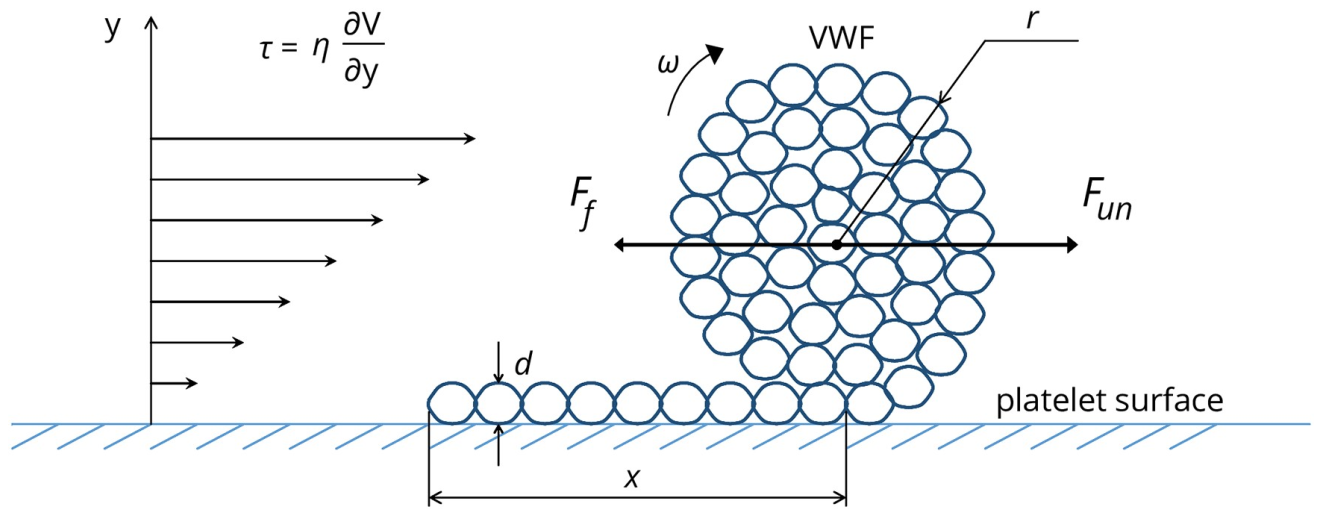
\includegraphics[width=0.6\textwidth]{./images/slides/vWF_unfolding.png}
    \end{center}
\end{frame}

\begin{frame}{\subsecname}
    \begin{columns}[T]
        \begin{column}{0.4\textwidth}
            Слипание тромбоцитов, однако, наблюдается при сдвиговых напряжениях,
            недостаточных для существенного разворачивания фактора~\cite{savage1996platelet_adhesion, rahman2019platelet_adhesion}.
        \end{column}

        \begin{column}{0.6\textwidth}
            \begin{figure}[ht!]
                \centering
                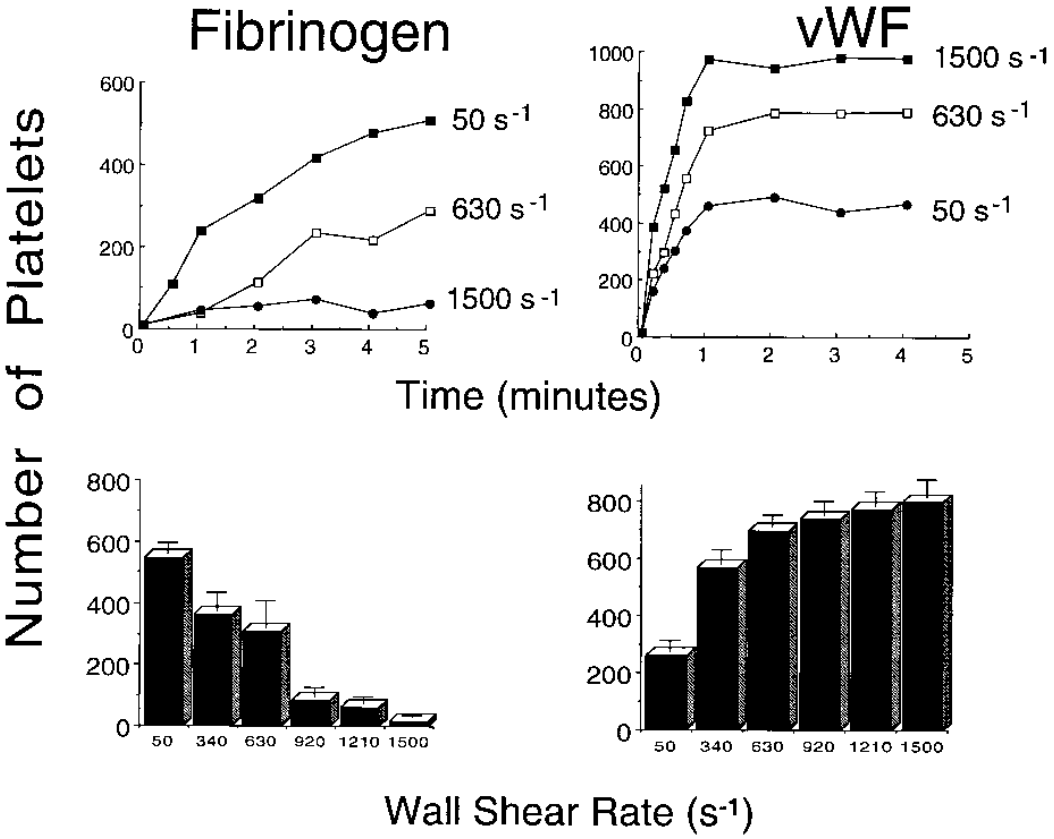
\includegraphics[width=0.8\textwidth]{./images/slides/Savage_platelets.png}
                \caption{Число налипших тромбоцитов из работы \textcite{savage1996platelet_adhesion}}
            \end{figure}
        \end{column}
    \end{columns}
\end{frame}

% \begin{frame}{\subsecname}
%     Тромбоцитарный тромб является
%     \begin{itemize}
%         \item подвижным~\cite{savage1996platelet_adhesion,jamiolkowski2016visualization};
%         \item пластичным~\cite{jamiolkowski2016visualization};
%         \item пористым~\cite{wufsus2013clot_permeability}.
%     \end{itemize}
% \end{frame}

\begin{frame}{\subsecname}
    Некоторые существующие модели:
    \begin{itemize}
        \item \fullcite{sorensen1999platelets_deposition_model}
        \item \fullcite{goodman2005thrombosis_model}
        \item \fullcite{wu2017deposition_model}
    \end{itemize}
\end{frame}

\begin{frame}{\subsecname}
    \centering
    \begin{figure}[ht!]
        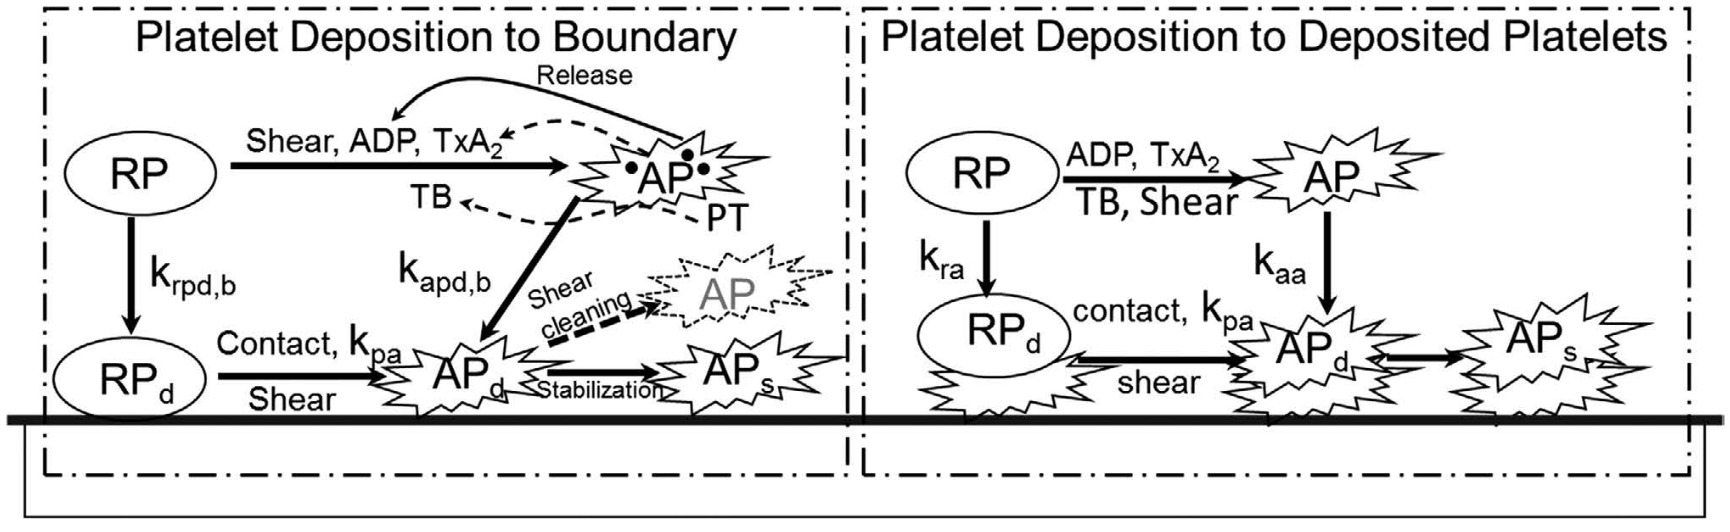
\includegraphics[width=1.0\textwidth]{./images/slides/wu_model.png}
        \caption{Иллюстрация к модели из работы \textcite{wu2017deposition_model}}
    \end{figure}
\end{frame}

\begin{frame}{\subsecname}
    Разработка новой модели мотивирована
    \only<1>{
        \begin{itemize}
            \item необходимостью интеграции существующей модели образования фибринового тромба;
            \item желанием использовать меньше компонент для описания выпадения и слипания тромбоцитов;
        \end{itemize}
    }
    \only<2>{
        \begin{itemize}
            \item желанием описывать слипание тромбоцитов посредством меняющейся проницаемости или вязкости;
            \item желанием учесть новые модели разворачивания фактора фон Виллебранда.
        \end{itemize}
    }
\end{frame}

\subsection{Модель тромбоцитарного тромба}

\begin{frame}{\subsecname}
    Добавим компартменты $ \phi_a $, $ \phi_d $~--- липкие и слипшиеся тромбоциты,
    соответственно. Липкие тромбоциты моделируются пассивной примесью, слипшиеся~--- неподвижны.

    Липкие налипают на стенку или на слипшиеся тромбоциты.
    Под действием сдвигового напряжения может происходить расцепление тромбоцитов.
    \[
        \begin{cases}
            \frac{\partial \phi_f}{\partial t} &= -k_{f \to a} \cdot \phi_f + k_{\mathrm{da}} \cdot \phi_a \\
            \frac{\partial \phi_a}{\partial t} &=  k_{f \to a} \cdot \phi_f - k_{a \to d} \cdot \phi_a + k_{\mathrm{da}} \cdot (\phi_d - \phi_a) \\
            \frac{\partial \phi_d}{\partial t} &=  k_{a \to d} \cdot \phi_a - k_{\mathrm{da}} \cdot \phi_d \\
        \end{cases}
    \]
\end{frame}

\begin{frame}{\subsecname}
    Предполагая объёмную концентрацию $ \phi_a $ постоянной (равновесной),
    можно аналитически решить уравнения реакции для зависимости $ \phi_d $ от времени:

    \begin{multline*}
        \frac{\partial \phi_d}{\partial t} = k_{a \to d} \cdot \phi_a - k_{\mathrm{da}} \cdot \phi_d
        \quad \Longrightarrow \\ \Longrightarrow \quad \phi_d(t) = \phi_a \frac{k_{a \to d}}{k_\mathrm{da}} - e^{-k_{\mathrm{da}}} \left( \phi_a \frac{k_{a \to d}}{k_\mathrm{da}} - \phi_d(0) \right)
    \end{multline*}
\end{frame}

\begin{frame}[fragile]
    \begin{figure}[ht!]
        \centering
        \small
        \begin{gnuplot}[terminal=tikz, terminaloptions={color size 14.0cm,6.7cm fontscale 0.7}]
            load './gnuplot/common.gp'

            set datafile separator ' '
            set key vertical maxrows 6 spacing 1.4

            set style increment default
            set style data lines
            set xlabel  "$ t, \\; \\textnormal{мин} $"
            set xrange  [ 0 : 5 ] noreverse writeback
            set ylabel  "$ N_{\\textnormal{тромбоцитов}}, \\; \\textnormal{шт.} $" offset -1 #rotate by 0
            set yrange  [ 0 : 1600 ] noreverse writeback

            # Модель
            f(a, k, x) = a * (1.0 - exp(-k * x))

            set xtics 1
            #set xzeroaxis lw 2

            plot "./data/platelets/Savage_fibrinogen_50_time_data.csv"   using 1:2 with points ps 3 t "Фибриноген, $ 50 \\; \\textnormal{с}^{-1} $", \
                "./data/platelets/Savage_fibrinogen_630_time_data.csv"  using 1:2 with points ps 3 t "Фибриноген, $ 630 \\; \\textnormal{с}^{-1} $", \
                "./data/platelets/Savage_fibrinogen_1500_time_data.csv" using 1:2 with points ps 3 t "Фибриноген, $ 1500 \\; \\textnormal{с}^{-1} $", \
                "./data/platelets/Savage_vWF_50_time_data.csv"          using 1:2 with points ps 3 t "vWF, $ 50 \\; \\textnormal{с}^{-1} $", \
                "./data/platelets/Savage_vWF_630_time_data.csv"         using 1:2 with points ps 3 t "vWF, $ 630 \\; \\textnormal{с}^{-1} $", \
                "./data/platelets/Savage_vWF_1500_time_data.csv"        using 1:2 with points ps 3 t "vWF, $ 1500 \\; \\textnormal{с}^{-1} $", \
                f(556.11,  0.4353, x) with lines lc 1 lw 2 t "$ k_\\mathrm{da} = 7.25 \\cdot 10^{-3} \\; \\textnormal{с}^{-1} $", \
                f(2013.02, 0.0296, x) with lines lc 2 lw 2 t "$ k_\\mathrm{da} = 4.92 \\cdot 10^{-4} \\; \\textnormal{с}^{-1} $", \
                f(44.27,   2.2744, x) with lines lc 3 lw 2 t "$ k_\\mathrm{da} = 3.71 \\cdot 10^{-2} \\; \\textnormal{с}^{-1} $", \
                f(460.91,  2.1932, x) with lines lc 4 lw 2 t "$ k_\\mathrm{da} = 3.65 \\cdot 10^{-2} \\; \\textnormal{с}^{-1} $", \
                f(799.96,  1.6614, x) with lines lc 5 lw 2 t "$ k_\\mathrm{da} = 2.76 \\cdot 10^{-2} \\; \\textnormal{с}^{-1} $", \
                f(980.54,  2.4312, x) with lines lc 6 lw 2 t "$ k_\\mathrm{da} = 4.05 \\cdot 10^{-2} \\; \\textnormal{с}^{-1} $"
        \end{gnuplot}
        \vspace{-1.5\baselineskip}
        \caption{Зависимость числа налипших тромбоцитов от времени при разной сдвиговой скорости в потоке у стенки~\cite{savage1996platelet_adhesion}.}
        \label{fig:reactions:vWF_platelets_count_time}
    \end{figure}
\end{frame}

\begin{frame}[fragile]
    \begin{figure}[ht!]
        \centering
        \small
        \begin{gnuplot}[terminal=tikz, terminaloptions={color size 14.0cm,6.7cm fontscale 0.7}]
            load './gnuplot/common.gp'

            set datafile separator ' '

            set style increment default
            set style data lines
            set xlabel  "$ \\dot \\gamma, \\; \\textnormal{с}^{-1} $"
            set xrange  [ 0 : 1600 ] noreverse writeback
            set ylabel  "$ N_{\\textnormal{тромбоцитов}}, \\; \\textnormal{шт.} $" offset -1 #rotate by 0
            set yrange  [ 0 : 1000 ] noreverse writeback

            # Модель
            f(x) = 805.7 * (1.0 - 0.759 * exp(-2.845e-3 * x))

            set xtics 200
            #set xzeroaxis lw 2

            plot "./data/platelets/Savage_data.csv" using 1:3 with points ps 3 t "экспериментальные данные \\cite{savage1996platelet_adhesion}", \
                f(x) with lines lw 3 t "экспоненциальная модель"
        \end{gnuplot}
        \vspace{-1.5\baselineskip}
        \caption{Зависимость числа налипших тромбоцитов от сдвиговой скорости в потоке у стенки~\cite{savage1996platelet_adhesion}.}
        \label{fig:reactions:vWF_platelets_count}
    \end{figure}
\end{frame}

\begin{frame}{\subsecname}
    Стоит учесть, что связи образуются только на определённом характерном расстоянии между тромбоцитами.

    Из предположения о равномерном распределении тромбоцитов в объёме при маленькой концентрации
    можно получить <<функцию активации>> связей.

    Для этого решается задача о расстоянии $ r_k $ до $ k $-ого ближайшего соседа.
    \[
        \mathbb{P} \{r_k < x\} = \mathbb{P} \left\{\textnormal{в $ V = V_{\text{ball}}(x) $ находится $ \geqslant k $ частиц} \right\}
    \]
\end{frame}

\begin{frame}{\subsecname}
    Функция распределения и функция плотности находятся из распределения Пуассона варьированием радиуса шара,
    в котором рассматривается число частиц
    \begin{align*}
        F_{r_k}(x) &= 1 - e^{- V(x) n} \sum_{m = 0}^{k-1} \frac{(V(x) n)^m}{m!} \\
        \rho_{r_k}(x)  &= S(x) n \cdot e^{-V(x) n} \frac{(V(x) n)^{k-1}}{(k-1)!}
    \end{align*}
    где $ V(x) $, $ S(x) $~--- функции объёма и площади поверхности шара радиуса $ x $.
\end{frame}

\begin{frame}{\subsecname}
    Функция распределения ведёт себя как гладкая ступенька.

    Считая, что тромб становится вязким в момент,
    когда характерное расстояния до нескольких ближайших соседей становится сравнимо с длиной фактора фон Виллебранда,
    получаем модификацию модели вязкости.
    \[
        \nu = \nu_{\text{blood}} \cdot (1 + F_{r_k}(L_{\text{vWF}}; n=\phi_{\text{d}}) \cdot \phi_{\text{d}} K (\dot \gamma)^{n-1})
    \]
\end{frame}


\subsection{Численные эксперименты}

\begin{frame}{\subsecname}
    \begin{figure}[ht!]
        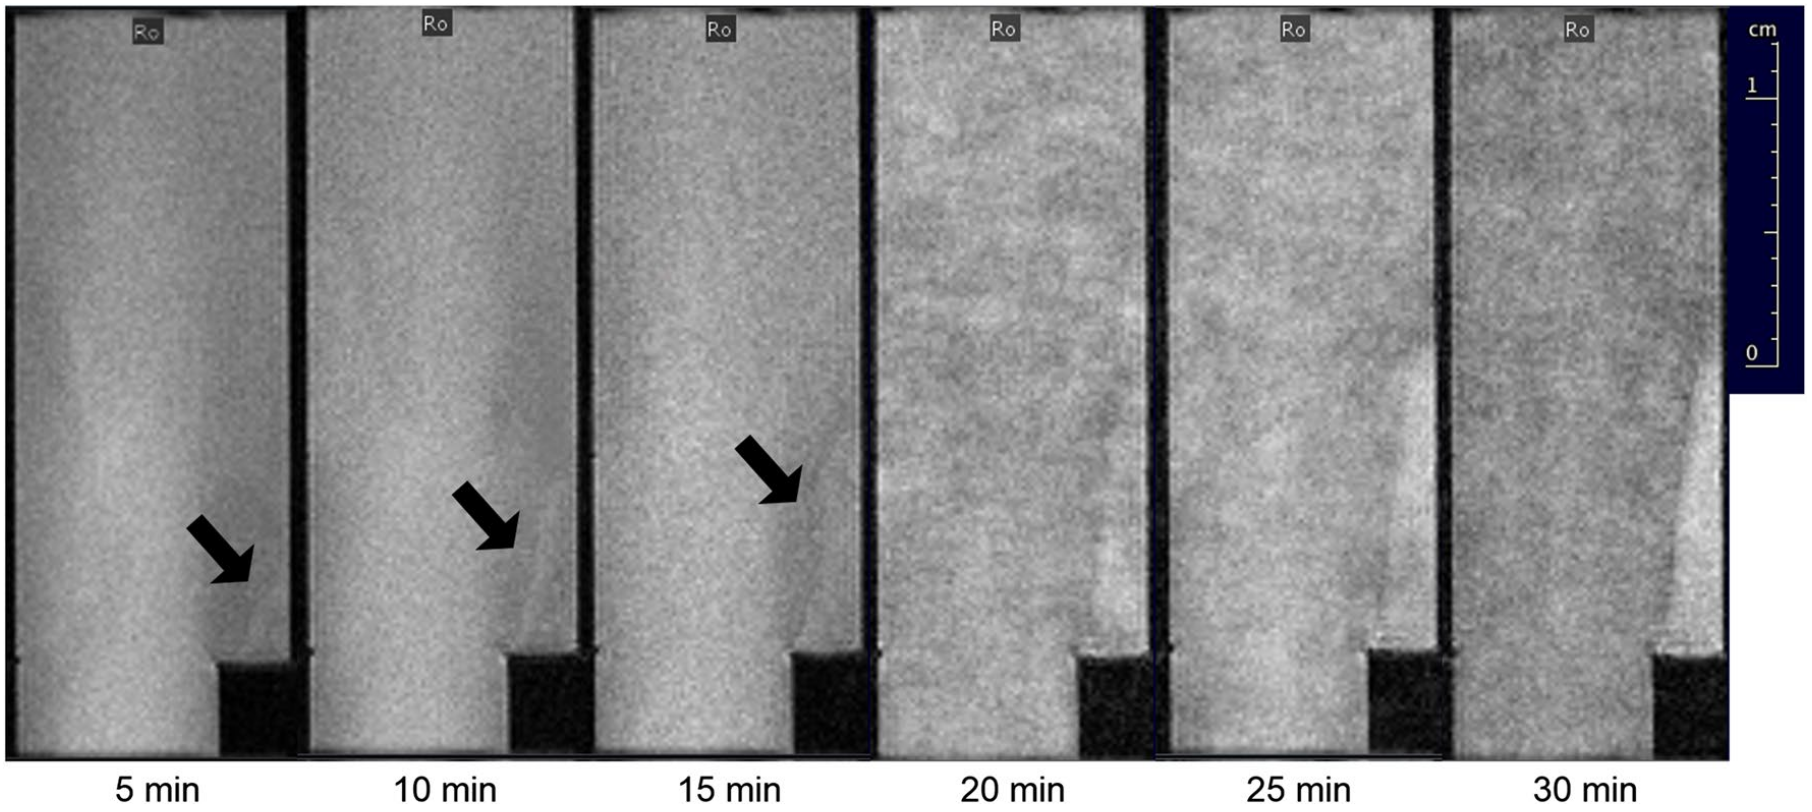
\includegraphics[width=0.9\textwidth]{./images/slides/yang_experiment.png}
        \caption{Рост тромба в трубке со ступенькой из работы \textcite{yang2021thrombosis_imaging}.}
    \end{figure}
\end{frame}

\begin{frame}
    \begin{columns}[T]
        \begin{column}{0.3\textwidth}
            \centering
            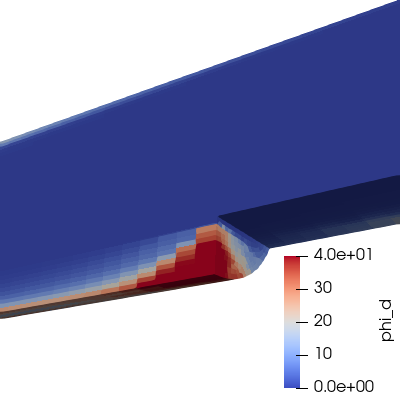
\includegraphics[width=1.0\textwidth]{./images/slides/blood_step_1.png}
        \end{column}
        \begin{column}{0.7\textwidth}
            \centering
            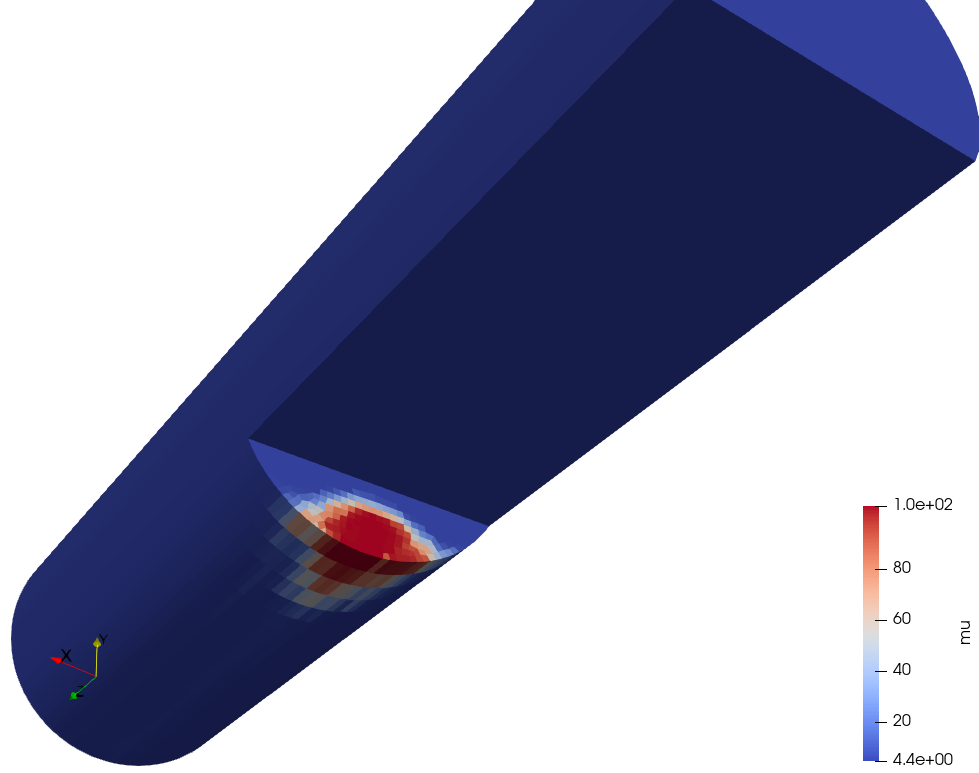
\includegraphics[width=1.0\textwidth]{./images/slides/blood_step_2.png}
        \end{column}
    \end{columns}
\end{frame}


\section{Метод адаптации численной схемы}

\begin{frame}{Каскад реакций~--- жёсткая система}
    При численном интегрировании модели каскада свёртывания крови
    неявные методы могут давать нефизичные решения (отрицательные концентрации).\footnote{\textcite{vassilevski2020parallel, butakov2022two_methods}}
\end{frame}

\begin{frame}{Существующие подходы}
    \begin{itemize}
        \item<1-> <<Классическая>> жёсткость устраняется устойчивыми неявными численными схемами.
        \item Экспоненциальные интеграторы позволяют точно интегрировать линейную часть системы.
    \end{itemize}
    \onslide<2->{
        Проблемы:
        \begin{itemize}
            \item Неявные схемы <<транслируют>> нелинейность правой части СОДУ на дискретизованное уравнение.
            \item Экспоненциальные интеграторы плохо справляются с нелинейной реакцией системы на малые возмущения.
        \end{itemize}
    }
\end{frame}

\begin{frame}{Существующие подходы}
    Можно ли совместить экспоненциальные интеграторы и неявные схемы?
    \begin{itemize}
        \item Методы Лоусона: замена переменных + стандартная численная схема.
            \[
                \bvec{v}(t) = \exp\left((t_{n-1} - t) \cdot \frac{\partial f}{\partial \bvec{x}}\right) \bvec{x}(t)
            \]
        \item Методы групп Ли.
        \item Некоторые существующие экспоненциальные интеграторы.
    \end{itemize}
\end{frame}

\begin{frame}{\secname}
    Предлагается динамически адаптировать существующие семейства численных методов для достижения
    \textbf{баланса между устойчивостью схемы и простотой поиска корней невязки}.
\end{frame}

\subsection{Методы Рунге-Кутты}

\begin{frame}{\subsecname}
    Полностью задаются матрицей $ \mathrm{A} $ и вектором $ \mathrm{b} $:
    \begin{align*}
        \mathbf{x}^{n+1} &= \mathbf{x}^n + \Delta t \sum_{m=1}^s b_m \mathbf{k}_m \\
        \mathbf{k}_m &= f \left( \mathbf{x}^n + \Delta t \sum_{j = 1}^s a_{ij} \mathbf{k}_j \right)
    \end{align*}
\end{frame}

\begin{frame}{\subsecname}
    Если правая часть линейна по $ \bvec{x} $, численное решение можно представить в виде
    \[
        \mathbf{x}^{n+1} = R \left( \Delta t \frac{\partial f}{\partial \mathbf{x}} \right) \mathbf{x}^n
        \qquad
        R(z) = \frac{\det \left(I - z \mathrm{A} + z e \mathrm{b}^T \right)}{\det \left(I - z \mathrm{A} \right)}
    \]
    Подберём $ \mathrm{A} $, $ \mathrm{b} $ так, чтобы воспроизводилось точное решение:
\end{frame}

\begin{frame}{Взвешенный метод Эйлера}
    Рассмотрим тета-схему:
    \[
        \begin{array}{c|cc}
            0 & 0 & 0 \\
            1 & 1 - \Theta & \Theta \\
            \hline
             & 1 - \Theta & \Theta
        \end{array}
    \]
    Воспользовавшись предложенным методом, получаем
    \[
        \Theta^\optimal(z) = \frac{1}{z} - \frac{1}{e^z - 1} = \frac{1}{2} - \frac{z}{12} + \frac{z^3}{720} + \Oclass(z^4)
    \]
\end{frame}

\begin{frame}{Система ван дер Поля (первая компонента)}
    \begin{center}
        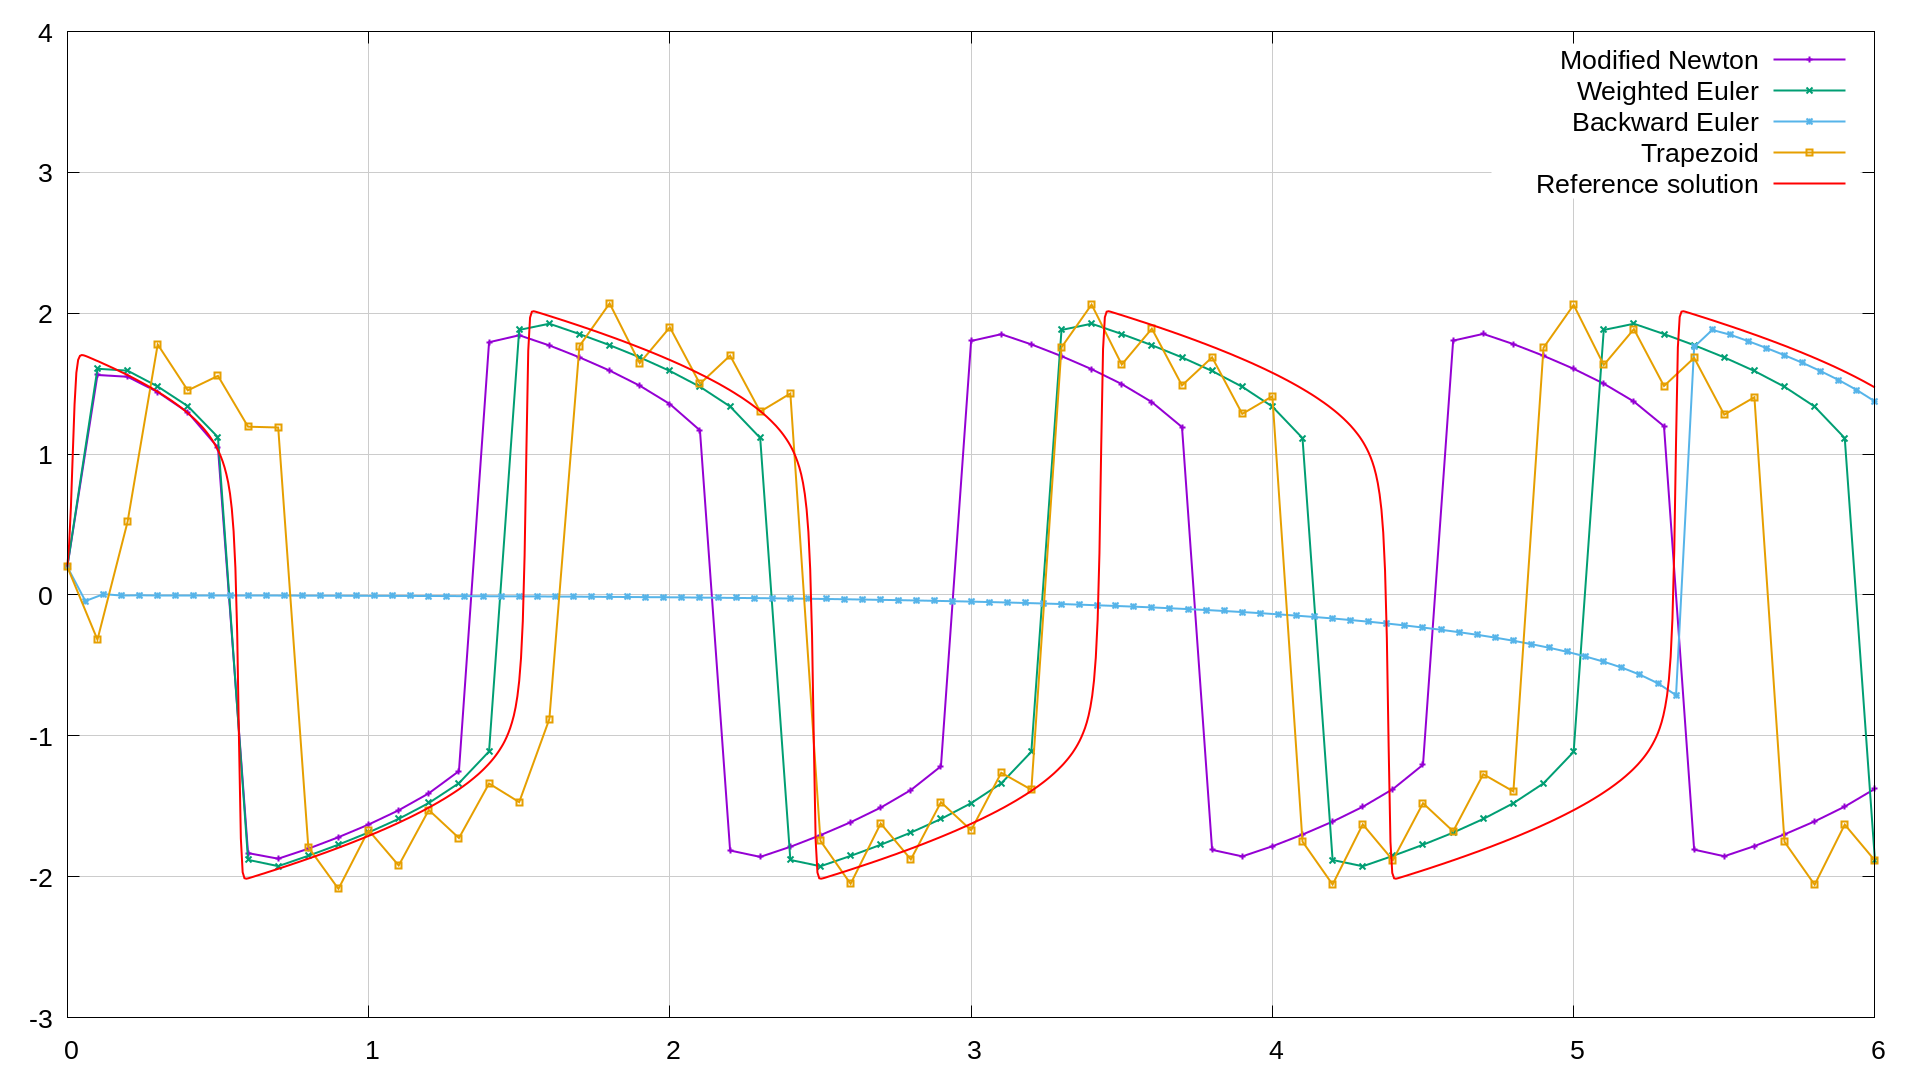
\includegraphics[width=0.85\textwidth]{./images/slides/van_der_Pol.png}

        \vspace{-1.0\baselineskip}
        {\tiny $ t $, у.е.}
    \end{center}
\end{frame}

\begin{frame}{Система ван дер Поля (первая компонента)}
    \begin{center}
        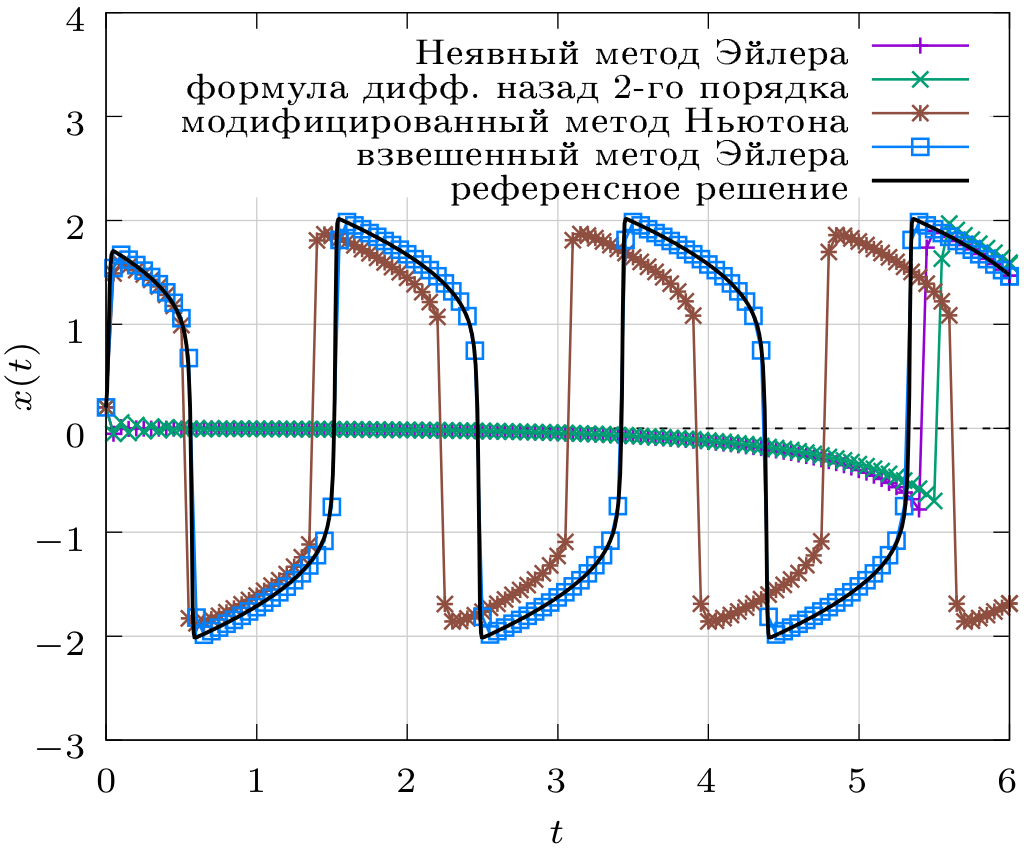
\includegraphics[width=0.48\textwidth]{./images/slides/van_der_Pol_1.png}
        \hfill
        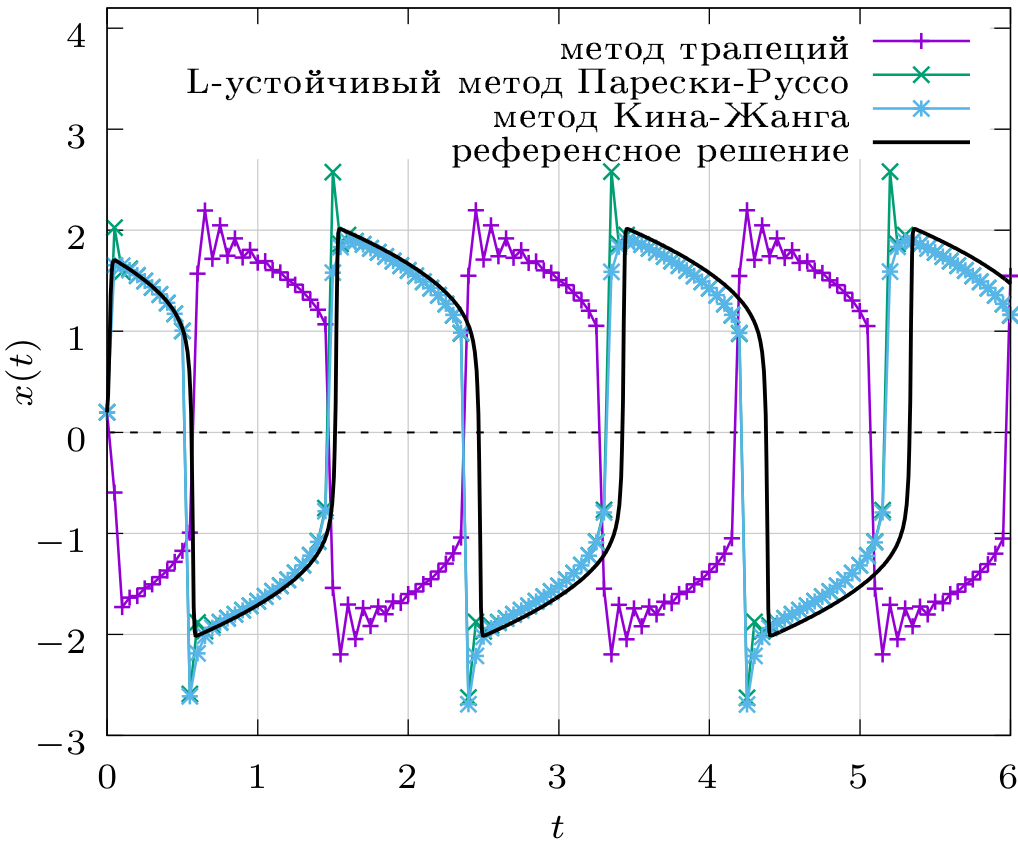
\includegraphics[width=0.48\textwidth]{./images/slides/van_der_Pol_2.png}
    \end{center}
\end{frame}

\begin{frame}[c]{Каскад свёртывания крови (тромбин)}
    \begin{center}
        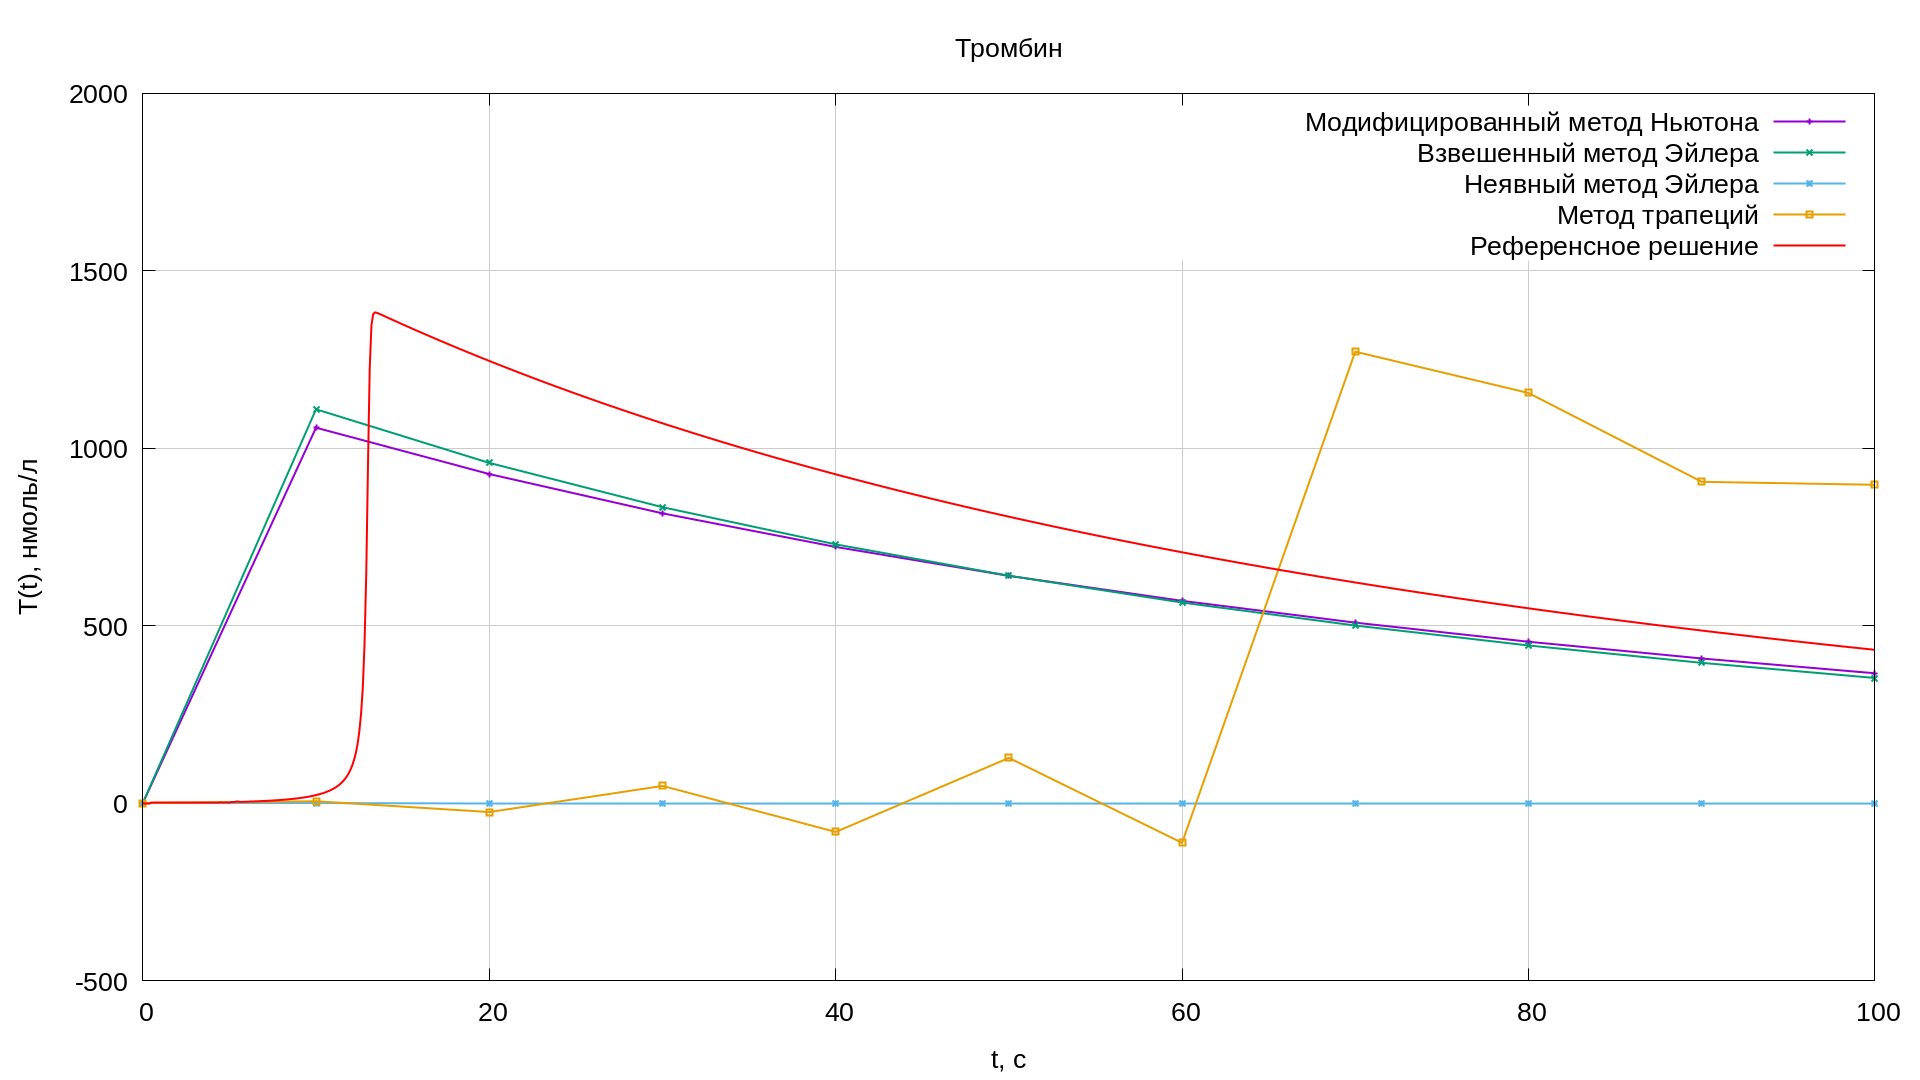
\includegraphics[width=0.91\textwidth]{./images/slides/thrombin.png}
    \end{center}
\end{frame}

% \begin{frame}{Дважды взвешенный метод Эйлера}
%     Рассмотрим следующее семейство двухстадийных методов Рунге-Кутты,
%     заданное таблицей Бутчера
%     \[
%         \begin{array}{c|cc}
%             0 & 0 & 0 \\
%             1 & 1 - \alpha & \alpha \\
%             \hline
%              & 1 - \beta & \beta
%         \end{array}
%         \qquad
%         \alpha, \beta \in \reals
%     \]
%     Поскольку параметра два, можно произвести подгонку под две экспоненты:
%     \[
%         R(z) = \exp(z), \quad R(x) = \exp(x), \quad x \neq z
%     \]
% \end{frame}
% 
% \begin{frame}{Дважды взвешенный метод Эйлера}
%     \[
%         \begin{aligned}
%             \alpha^\optimal(x,z) &= \frac{z^2 (e^x - 1 - x) - x^2 (e^z - 1 - z)}{x z( z (e^x - 1) - x (e^z - 1))} \approx \frac{1}{3} - \frac{x + z}{36} \\
%             \beta^\optimal(x,z)  &= \frac{(x-z)(e^z - 1 - z)(e^x - 1 - x)}{x z (z(e^x - 1) - x (e^z - 1))} \approx \frac{1}{2} + \frac{x + z}{6}
%         \end{aligned}
%     \]
%     В пределе сильно диссипативной системы имеем взвешенный метод Эйлера:
%     \[
%         \lim_{x \to -\infty} \alpha^\optimal(x,z) = \lim_{x \to -\infty} \beta^\optimal(x,z) = \Theta^\optimal(z)
%     \]
% \end{frame}
% 
% \begin{frame}{Дважды взвешенный метод Эйлера}
%     \textbf{Проблема:} $ x $ и $ z $ могут не коммутировать.\newline
%     \textbf{Решение:} $ x \approx \identity \cdot (\trace x / d) $.
% 
%     \textbf{Проблема:} $ x $ и $ z $ могут быть близки к нулю.\newline
%     \textbf{Решение:} разложение в ряд Тейлора.
% 
%     \textbf{Проблема:} $ x $ и $ z $ могут быть близки друг к другу.\newline
%     \textbf{Решение:} $ x = z + \delta $ и разложение в ряд Тейлора.
% \end{frame}
% 
% \begin{frame}{Система ван дер Поля (первая компонента)}
%     \begin{center}
%         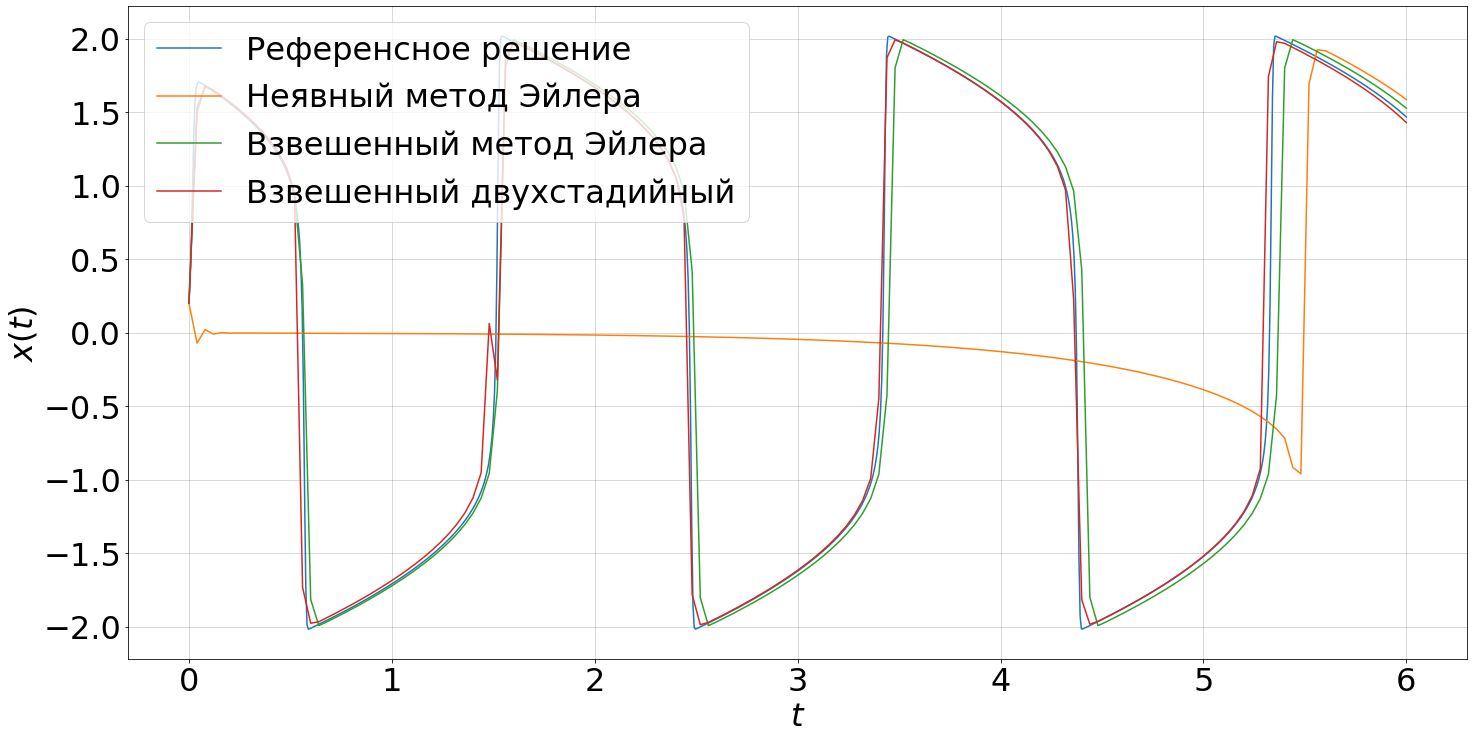
\includegraphics[width=0.95\textwidth]{./images/slides/van_der_Pol_double.png}
%     \end{center}
% \end{frame}
% 
% \begin{frame}{Адаптированный двухстадийный SDIRK-метод}
%     Рассмотрим следующее семейство двухстадийных SDIRK-методов Рунге-Кутты~\cite{franko1997SDIRK},
%     заданное таблицей Бутчера
%     \[
%         \begin{array}{c|cc}
%             \alpha & \alpha & 0 \\
%             1      & 1 - \alpha & \alpha \\
%             \hline
%             & 1 - \alpha & \alpha
%         \end{array}
%         \qquad
%         \alpha \in \reals
%     \]
%     Воспользовавшись предложенным методом, получаем
%     \[
%         \alpha^\optimal(z) = \frac{1 - e^{-z}}{z} \pm e^{-z} \sqrt{\frac{1}{z^2} \left( e^z (z - 1) + 1 \right)}
%     \]
% \end{frame}
% 
% \begin{frame}{Ограничения и дополнительные результаты}
%     Ограничения:
%     \begin{itemize}
%         \item
%             Требуется считать функцию от матрицы.
%             Возможное решение~--- применять функцию к усреднённому спектру ($ \trace A / d $).
%         \item
%             Неоднозначность выбора точки, в которой производится линеаризация.
%     \end{itemize}
% 
%     Дополнителльные результаты:
%     \begin{itemize}
%         \item
%             В работе метод был опробован и на других задачах,
%             имеющих аналитическое решение (логистический рост, задача двух тел)
%     \end{itemize}
% \end{frame}

\begin{frame}{Заключение}
    Сделаны первые шаги к построению новой модели белого тромба;
    модель воспроизводит начальную стадию образования тромба в тесте со <<ступенькой>>.
    Основное ограничение~--- все компоненты моделируются пассивной примесью.

    Также разраюатывается вариант модели с неподвижными налипшими тромбоцитами.

    Развит ранее предложенный и разработан новый метод вариации коэффициентов численной схемы
    с целью получения точных интеграторов.
    Приведены примеры, соответствующий анализ и эксперименты.
\end{frame}

\begin{frame}[allowframebreaks]
    \printbibliography
\end{frame}


\end{document}
